%!TEX root = ../rapport.tex
%!TEX encoding = UTF-8 Unicode

% Chapitres "Introduction"

% modifié par Francis Valois, Université Laval
% 31/01/2011 - version 1.0 - Création du document

\chapter{Schémas électroniques 1$^{ère}$ itération}
\label{electronics}

\begin{figure}[htbp]
\centering
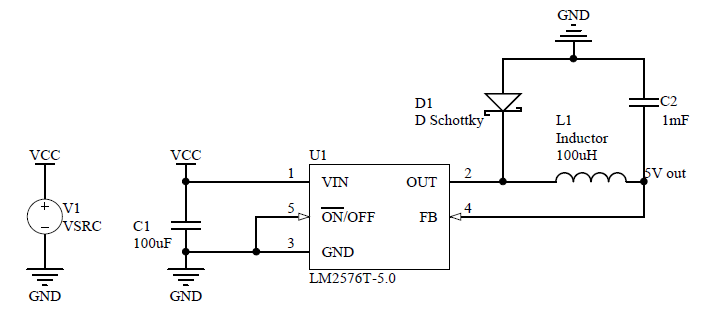
\includegraphics[scale=0.5]{fig/alim_5V.png}
\caption{Figure présentant les plans de l'alimentation 5V pour les périphériques}
\label{fig:alim5V}
\end{figure}

\begin{figure}[htbp]
\centering
\includegraphics[scale=0.1]{fig/alim_24V_photo.png}
\caption{Figure présentant une photo de l'alimentation 24V pour les périphériques}
\label{fig:alim24Vphoto}
\end{figure}

\begin{figure}[htbp]
\centering
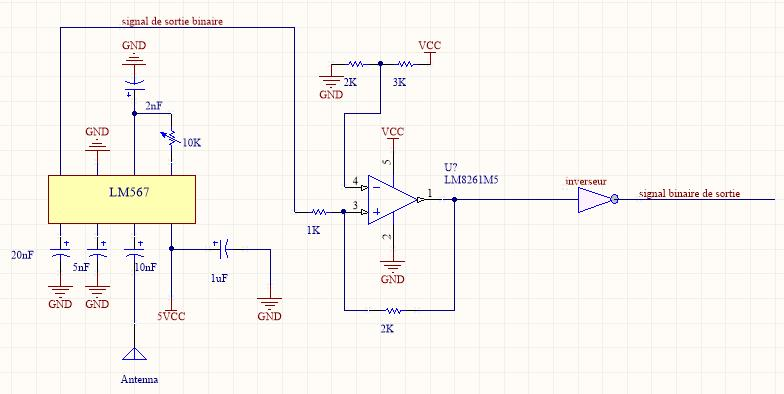
\includegraphics[scale=0.5]{fig/circuit_manchester.jpg}
\caption{Figure présentant les plans du récepteur Manchester}
\label{fig:manchester}
\end{figure}

\begin{figure}[htbp]
\centering
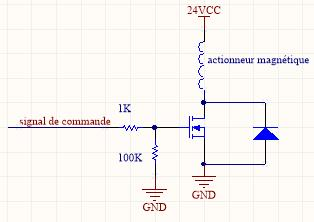
\includegraphics[scale=0.5]{fig/prehenseur.jpg}
\caption{Figure présentant les plans du circuit de commande du préhenseur}
\label{fig:prehenseur}
\end{figure}

\begin{figure}[htbp]
\centering
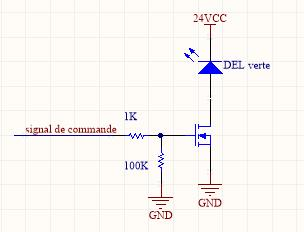
\includegraphics[scale=0.5]{fig/del_verte.jpg}
\caption{Figure présentant les plans du circuit de commande du préhenseur}
\label{fig:del_verte}
\end{figure}